\documentclass[acmtog,review]{acmart}

\usepackage{booktabs} % For formal tables

\settopmatter{printacmref=false} % Removes citation info after abstract
\renewcommand\footnotetextcopyrightpermission[1]{} % removes footnote with conference information in first column
\usepackage{fancyhdr}
\usepackage{url}
 
\pagestyle{fancy}
\fancyhf{}
\rfoot{\thepage}

%\pagestyle{plain} % removes running headers

% Use the "authoryear" citation style, and make sure citations are in [square brackets].
\citestyle{acmauthoryear}
\setcitestyle{square}

% A useful command for controlling the number of authors per row.
% The default value of "authorsperrow" is 2.
\settopmatter{authorsperrow=4}

\begin{document}

% Title. 
% If your title is long, consider \title[short title]{full title} - "short title" will be used for running heads.
\title{The Probability of Winning at Blackjack}
\subtitle{Research Design, Amsterdam, September 2019}

% Author
\author{Robin Vonk}
\affiliation{%
  \institution{Amsterdam University of Applied Sciences}}

\maketitle

% a couple of paragraphs describing your project
\section*{Abstract}
This paper takes a look at the game played at every casino over the world, Blackjack. Results are gathered by simulation games of Blackjack in a Python program. With this approach a very large dataset can be generated in a matter of minutes. The following questions will be answered: 
\begin{itemize}
  \item What is the best move a player in Blackjack can make, for each possible value in his hand?
  \item "The dealer wins, overall, more games than the player", is that true?
\end{itemize}
This is tested with a generated dataset with the results of one million games of Blackjack. After refining the data it results in that the dealer indeed wins more games than the player. In total about 22 percent more games to be exact. \\
This refinement also shows that when the player does the following moves with the corresponding hand value, this will result in the highest probability to win:
\begin{itemize}
    \item < 12: Draw
    \item 12: Draw
    \item 13: Draw
    \item 14: Draw
    \item 15: Pass
    \item 16: Pass
    \item 17: Pass
    \item > 17: Pass
\end{itemize}


% the other sections
\section{Introduction}
For experienced Blackjack players it won't be difficult to make the correct move with most hands of cards. \\
 \\
For example when the player gets 18, 19 or 20 in his starting hand, the player will always pass. If the player chooses to draw a card, the probability is very high he will lose. \\
Another example, when the player gets 9, 10 or 11 in his hand, he will always at least draw one extra card. This is because the player can\textquotesingle t go over 21 with 1 more card and the probability of winning with this starting hand is very low. \\
However when the player gets 14, 15 or 16 in his hand, things get more difficult. One more card can be fatal, but not drawing a card has a big probability of losing from the dealer. \\
 \\
This paper will discuss what the best move is with these difficult hands. The way this is tested is by playing many games of Blackjack and writing down the results. The result with the most wins, wins! However to be able to get a reliable result, we will need a lot of data. A few games will not give a reliable reflection of the probability of the game, because it could be coincidence. With coincidence is meant, when four games are played and all four are won by the player, this is coincidence. It is not a good reflection of the reality, but a result of random factor. In the case of Blackjack is the random factor the cards which are randomly shuffles. No matter how big the data set gets, we will always keep a coincidence. The probability will always exists that the player or dealer wins more games in the test than he will in reality. However this probability can be made smaller and smaller by expanding the dataset. This is why the experiment is done with a simulation of Blackjack in the programming language Python. With the power of computers, thousands of games of Blackjack can be played each second! With this approach is expected that it will minimize the coincidence and the results will be reliable. \\
With all the results of the games it is possible to extract the decisions the player made combined with how many times the player won and lost, resulting in which move gives the highest probability to win. \\
 \\
Another thing that will be looked at is the total wins of the dealer and the total wins of the player and the ratio between these. Expected is that, with the normal Blackjack rules used in the casino, the dealer will have a higher number of wins. If this is not the case, it wouldn't make sense for casinos to play this game. They would only be losing money in the long run! \\
\section{The rules of Blackjack}
To understand this paper, it is important to understand the rules of Blackjack. This paper and the code to generate and refine the data is based around the most common rules used in casinos. \\
Blackjack is a card game which is played in casinos all around the world. It is an one versus one game with two players, the dealer and the player. The dealer deals the cards and the player decides what moves he wants to do. \\
 \\
The goal is for the player to have a higher card value than the dealer, without going over the value of 21. \\ 
The values of the cards are as followed: \\
Ace : 11 or 1 points \\
King, Queen, Jack : 10 points \\
2 to 10 : Its card value \\
 \\
The game starts with the dealer giving himself one card and the player two cards. All cards are open in Blackjack. The player has now two choices: He can either pass or draw. When the player draws he gets an extra card and gets to choose again. When the player passes, it is the turn of the dealer. The dealer draws cards until he has at least a value of 17 in his hand. After the dealer is done drawing cards, the value of the dealer is compared to the value of the player. The highest value wins, however if either value goes over 21, it automatically results in a lose for that side. An exact value of 21 results in an automatic win. 
\section{Experimental setup}
All code used for generating and refining data in this experiment is open-source and can be found on GitHub: \url{https://github.com/obin1000/Blackjack-DataResearch} \\
The experiment consists of two parts: \\
- Generating data \\
- Refining this data \\
 \\
Both parts make use of the programming language Python. \\
Generating the data is done by repeatedly playing games of Blackjack in a simulation. This results of the simulation are written to an .xlsx (Excel) file as storage. The hardest part in designing a simulator like this is, is how you will simulate the choices the player has to make. In the simulator for this experiment, the following rules are defined for the player:
\begin{enumerate}
  \item If the hand value is lower than 12, always draw a card. The player cannot lose by drawing one more card with a value lower than 12.
  \item If the hand value is higher than 17, always pass. There are few cards that the player can draw, that won't result in a value higher 21 in this case. \\
\end{enumerate}
So when the player gets an hand value between 11 and 18 he has two options, draw or pass. This decision is made randomly by the Python function randint(0,1), which generates a random number between 0 and 1. When it is an 1 the player draws a card and rolls again a new number for the next decision, when it is 0 the player passes.

Refining the data is done by scanning over the dataset that was created by the generator. While scanning it keeps track of the following counters:
\begin{itemize}
  \item The total number of wins by the dealer
  \item The total number of wins by the player
  \item The number of tied games
  \item For each hand value between 11 and 18:
    \begin{itemize}
        \item The value of the hand
        \item The total number of times the player decided to draw a card
        \item The number of wins by drawing a card
        \item The total number of times the player decided to pass
        \item The number of wins by passing
    \end{itemize}
\end{itemize}
The results of the refinement are written to a different .xlsx (Excel) sheet as storage (The Python library is not able to edit exsisting .xslx files, only create new ones). With this data it also automatically adds some graphs to display the data.

\section{Results}
The program was configured to generate a dataset of one million games of Blackjack. This number was chosen, because adding more 0\textquotesingle s to this number increases the time it takes to generate and refine the data set a lot. With one million it took my laptop approximately 5 minutes to generate and 1 minute to refine the data. I could wait longer for more data, but it is not expected to make a difference in the results. one million should be enough data to minimize the coincidence and give reliable results. \\
 \\
Figure 1 and table 1 show all hand values considered difficult with the total number of occurrences when
\begin{itemize}
    \item The player decided to draw 
    \item The player decided to pass
    \item The player decided to draw and won
    \item the player decided to pass and won 
\end{itemize}
An interesting trend appears in the graph with this data. You can see that, the higher the hand value, the less successful it is to draw a card (Blue in figure 1). So drawing a card with a hand value of 12 is more successful than drawing a card at a hand value of 17. This makes sense, because a lower hand value can draw more different cards without going over 21, so has a higher probability of winning.
The same happens to the passing card results, but in opposite order. The higher the hand value, the higher the probability passing will be successful (Red in figure 1). The interesting part in this graph is the differences between these two trends. For the outer two columns the results are very clear:
\begin{itemize}
    \item 12: Probability to win much better by drawing
    \item 13: Probability to win better by drawing
    \item 16: Probability to win better by passing
    \item 17: Probability to win way, way better by passing 
\end{itemize}
In the middle of the graph is the most important data. As expected are 14 and 15 the most difficult hands to make a decision for. When you look at the data it is slightly better to draw a card at a value of 14 and to pass at a value of 15. Based on the big dataset, it is safe to say that is also the best move in this situation. Making the right decision won\textquotesingle t make a big difference for your results while playing the game in real life, but if you happen to play one million games with a value of 14 or 15 in your hand, you could increase your win probability.

\begin{table}[H]
    \caption{Results per value}
\begin{tabular}{|l|l|l|l|l|l|l|}
\hline
 & 12 & 13 & 14 & 15 & 16 & 17 \\ \hline
Total times drawn  & 54477 & 54247 & 53520 & 54795 & 53285 & 47020 \\ \hline
Total times passed  & 57280 & 56577 & 56308 & 57379 & 54557 & 55578 \\ \hline
Total wins by drawing  & 18381 & 16983 & 15696 & 15014 & 14040 & 10255 \\ \hline
Total wins by passing  & 16120 & 16029 & 16032 & 16342 & 15660 & 20723 \\ \hline
\end{tabular}
\end{table}
\begin{figure}[H]
  \centering
  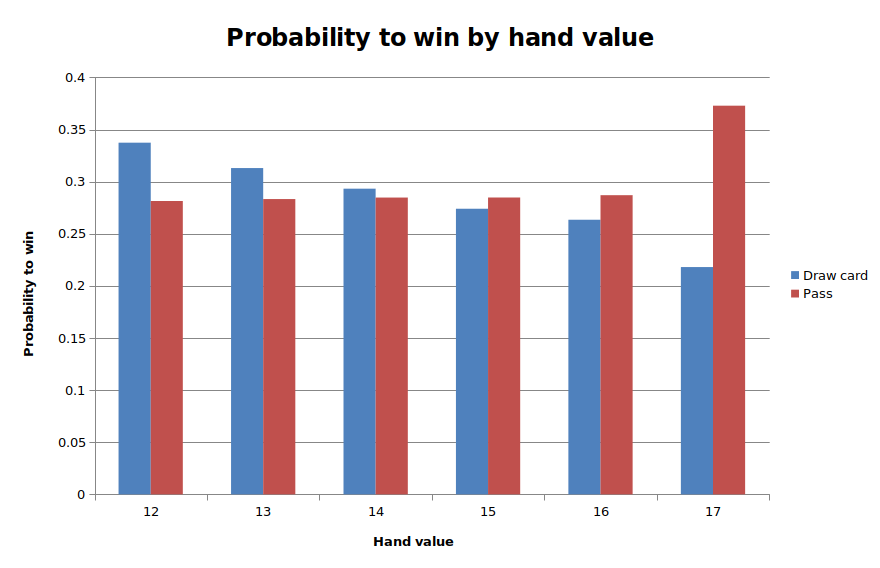
\includegraphics[width=\linewidth]{fig/GraphWinChanceCardValue.png}
  \caption{Graph showing the chance to win for the player by passing and drawing for each hand value in 1000000 games.}
\end{figure}


Figure 2 and table 2 show the total number of occurrences of each possible outcome over the entire experiment of one million games of Blackjack. You can see that the dealer won 513440 / 1000000 * 100 = 51,3 percent of the games, the player won 421942 / 1000000 * 100 = 42,2 percent of the games and only 64618 / 1000000 * 100 = 6,5 percent of the games resulted in a tie. This has a ratio of 1,22 / 1 / 0.15 with Dealer / Player / Tied. This means that, in the long run, the dealer always wins 1,22 times more games than the player. That is 22 percent more games.


\begin{table}[H]
    \caption{Total wins}
\begin{tabular}{|l|l|l|l|}
\hline
 & Dealer & Player & Tied \\ \hline
Total wins &  513440 & 421942 & 64618\\ \hline
\end{tabular}
\end{table}

\begin{figure}[H]
  \centering
  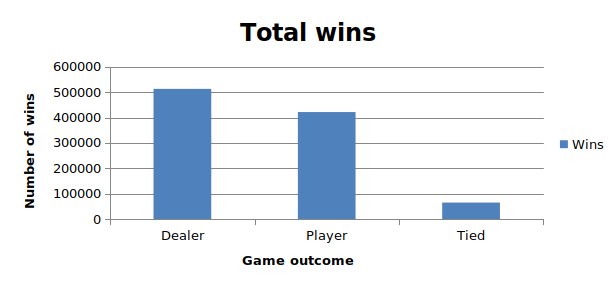
\includegraphics[width=\linewidth]{fig/GraphTotalWins.png}
  \caption{Graph showing total wins for player, dealer and ties in 1000000 games.}
\end{figure} 

\section{Conclusions and Future Work}
The goal of this research is to find out what the best move is in the casino game Blackjack with each hand value and to confirm the thought that the dealer always wins more games than the player. \\
First the total number of wins: The simulation of Blackjack gives an accurate representation of the game. After playing one million games in this simulation, it shows that the dealer indeed wins more games than the player. 22 percent more games to be exact in the case of this simulation. So this proves the hypothesis, in Blackjack, the dealer wins more games than the player. \\
\\
The best move for the player is the move with the highest probability to win. For the values bellow 12 and over 17 this is clear, draw if under 12 and pass if over 17. Between these values these choice gets more difficult. The results shows for 12 and 13 a clear advantage to draw a card and for 16 and 17 a clear advantage by passing. But for 14 and 15 things get very close. On the long run, one should draw a card with a value of 14 and pass at a value of 15. So in short:
\begin{itemize}
    \item < 12: Draw
    \item 12: Draw
    \item 13: Draw
    \item 14: Draw
    \item 15: Pass
    \item 16: Pass
    \item 17: Pass
    \item > 17: Pass
\end{itemize}
This paper is based on generation one time, one million games of Blackjack. To further proof the working of this experiment in more depth, one could generate multiple sets of one million games of Blackjack and compare the differences between these sets. Expected is that the differences between these sets should be minimal. The only differences in the data will be coincidences, which should be canceled out by the large size of the dataset.


\section{Discussion}
What could have gone wrong? \\
There are several factors on which this experiment could have gone wrong. First of all the program to generate the data uses the function shuffle() from the random library in Python. This function is used to shuffle the deck of cards. Due to computers cannot generate random numbers and I don't know how the shuffling is done in this function, I cannot know for sure that this function shuffles the deck in a reliable way. If the shuffle is not random, this can result in repetitive decks of cards, which games based on this deck would result in the same results, which could make the win probability turnout higher or lower than they really are. \\ 
This does not apply tot the randint() function from the same library, which is used for the user decision in drawing or passing. The counters in the refinement proof that this function gave a good 50/50 ratio in draw and pass, this is what it is intended to do.
 

% \begin{acks}
% The authors would like to thank \dots.
% \end{acks}

% select the reference format (leave this)
% \bibliographystyle{ACM-Reference-Format}

% specify the bibliography (.bib) file
% place your references in this bib file
% \bibliography{main}

\end{document}